%% ****** Start of file apstemplate.tex ****** %
%%
%%
%%   This file is part of the APS files in the REVTeX 4.2 distribution.%%
%%   Copyright (c) 2024 The American Physical Society.
%%
%%   See the REVTeX 4 README file for restrictions and more information.
%%
%
% This is a template for producing manuscripts for use with REVTEX 4.2
% Copy this file to another name and then work on that file.
% That way, you always have this original template file to use.
%
% Group addresses by affiliation; use superscriptaddress for long
% author lists, or if there are many overlapping affiliations.
%  N.B. The groupedaddress option will reorder the author list based
%  on the order in which affiliations appear. Please be sure to check the author 
%  order. You can also use the unsortedaddress(?) option instead to prevent that
%  behavior.
% For Phys. Rev. appearance, change preprint to twocolumn.
% Choose physrev, prl, or rmp for journal
%  N.B. physrev is appropriate for all APS journals except prl and rmp
%  Add 'draft' option to mark overfull boxes with black boxes
%  Add 'showkeys' option to make keywords appear
\documentclass[aps,physrev,preprint,groupedaddress,linenumbers]{revtex4-2}
%\documentclass[aps,physrev,preprint,superscriptaddress]{revtex4-2}
%\documentclass[aps,prl,preprint,superscriptaddress]{revtex4-2}
%\documentclass[aps,prl,reprint,groupedaddress]{revtex4-2}
%\documentclass[aps,rmp,preprint,superscriptaddress]{revtex4-2}
%\documentclass[aps,rmp,reprint,groupedaddress]{revtex4-2}

% You should use BibTeX and apsrev.bst for references
% Choosing a journal automatically selects the correct APS
% BibTeX style file (bst file), so only uncomment the line
% below if necessary.
\bibliographystyle{apsrev4-2}

% Packages
\usepackage{graphicx}
\usepackage{amsmath}
\usepackage{amssymb}
\usepackage[english]{babel}
\usepackage{hyperref}
\usepackage{xcolor}
\newcommand{\rev}[1]{{\color{blue}#1}}
\begin{document}

% Use the \preprint command to place your local institutional report
% number in the upper righthand corner of the title page in preprint mode.
% Multiple \preprint commands are allowed.
% Use the 'preprintnumbers' class option to override journal defaults
% to display numbers if necessary
%\preprint{}

%Title of paper
\title{\textbf{Scaling behaviors in simulated collagen fibrils}}

\author{Robert Bertoldo Tavares}
\affiliation{Departamento de Física, Universidade Federal do Ceará, Fortaleza, Ceará, Brasil}

\author{Michael Ferreira de Souza}
\affiliation{Departamento de Estatística e Matemática Aplicada, Universidade Federal do Ceará, Fortaleza, Ceará, Brasil}

\author{B\'ela Suki}
\affiliation{Department of Biomedical Engineering, Boston University, Boston, MA, USA}

\author{Ascânio Dias Araújo}
 \email{ascanio@fisica.ufc.br}
\affiliation{Departamento de Física, Universidade Federal do Ceará, Fortaleza, Ceará, Brasil}
\affiliation{Departamento de Estatística e Matemática Aplicada, Universidade Federal do Ceará, Fortaleza, Ceará, Brasil}

%Collaboration name if desired (requires use of superscriptaddress
%option in \documentclass). \noaffiliation is required (may also be
%used with the \author command).
%\collaboration can be followed by \email, \homepage, \thanks as well.
%\collaboration{}
%\noaffiliation

\date{\today}

\begin{abstract}
Collagen fibrils provide the primary source of tensile strength in mammalian connective tissues. Understanding how assembly kinetics dictate fibril architecture—and how that topology governs mechanical failure—is central to soft matter physics and bio-inspired material design. Here, we model collagen fibril formation using a modified diffusion-limited aggregation (DLA) framework where rod-like molecules undergo $T_{\mathrm{s}}$ surface-diffusion steps post-attachment, progressively compacting the structure. Coupling this morphological model with a probabilistic fracture framework reveals that $T_{\mathrm{s}}$ drives a structural crossover from porous fractal cross-sections to nearly space-filling architectures, with the fractal dimension $D_f$ rising monotonically from $1.708 \pm 0.005$ ($T_{\mathrm{s}} = 2$) to $1.963 \pm 0.001$ ($T_{\mathrm{s}} = 8192$). This compaction increases the mean rupture force $F_{\mathrm{r}}$ by an order of magnitude, with $83\%$ of the strength gain already realized at $T_{\mathrm{s}} = 128$. Mechanistically, failure is governed by two local structural variables set by $D_f$: the mean load-bearing cross-sectional count $\langle N \rangle$ and the molecular coordination number $\langle K \rangle$. In open fibrils ($D_f \approx 1.71$), severe cross-sectional heterogeneity induces localized stress concentrations and rapid $\langle K \rangle$ loss, sustaining extensive failure cascades ($\gamma = 2.00 \pm 0.013$). In compact fibrils ($D_f \to 2.0$), uniform packing preserves $>97\%$ of $\langle K_0 \rangle$ until failure, suppressing large cascades and steepening the power-law exponent to $\gamma = 2.55 \pm 0.008$. Across all architectures, pre-terminal damage remains bounded while final failure occurs via a single catastrophic cascade. These findings establish $D_f$ as an architectural bridge linking assembly kinetics to failure statistics, offering a mechanistic principle for designing resilient biological and synthetic fibers.\end{abstract}

% insert suggested keywords - APS authors don't need to do this
\keywords{Collagen, DLA, Fractals, Fracture, Avalanches}

%\maketitle must follow title, authors, abstract, and keywords
\maketitle

% body of paper here - Use proper section commands
% References should be done using the \cite, \ref, and \label commands
\section{Introduction}

Type I collagen is the principal structural protein of the mammalian extracellular matrix (ECM), providing essential mechanical integrity to tissues such as skin, tendon, bone, cartilage, and the cornea \cite{Silver2018,DavisonKotler2019,Tresoldi2013,Fedarko2014, RicoLlanos2021,Chen2015,Suki2021}. These hierarchical assemblies are critical for elasticity, tensile strength, and resilience against physical stress \cite{Silver2018,Amirrah2022}. Individual collagen molecules, characterized by a high aspect ratio ($\approx 300~\text{nm} \times 1.5~\text{nm}$) \cite{Gelse2003, Silver2018}, self-assemble into fibrils that can reach lengths of $500~\mu\text{m}$ and diameters of $500~\text{nm}$ \cite{Charvolin2019,Kadler1996, Parry1984}. These fibrils further aggregate into fibers ($1$--$20~\mu\text{m}$ diameter), forming a multiscale network capable of storing and transmitting mechanical energy \cite{Silver2008,Suki2021}.

Characterizing the mechanical behavior of collagen fibrils, particularly at the nanoscale, presents significant challenges \cite{Nalbach2022}. Experimental techniques such as atomic force microscopy (AFM) and micro-mechanical actuation have successfully probed the tensile properties of isolated fibrils. Van der Rijt et al. used AFM to measure the mechanical properties of tendon fibrils, evaluating their tensile behavior until failure \cite{vanderRijt2006}, while Svensson et al.~\cite{Svensson2018} developed a piezoelectric actuator-based technique to measure stress and strain during uniaxial stretching. However, resolving the collective molecular dynamics that govern failure remains difficult due to experimental resolution limits, particularly when characterizing small-scale forces and intermolecular interactions \cite{Andriotis2023}. Consequently, computational modeling has become indispensable for exploring the relationship between intrafibrillar organization and macroscopic mechanical response under a wider range of conditions.

Several theoretical frameworks have been developed to address fibril mechanics. Buehler et al. introduced coarse-grained molecular dynamics to model large-scale deformation, while Depalle et al. investigated the role of mineralization in stabilizing fibril elasticity in bone\cite{Buehler2006a,Buehler2006b,Buehler2008a,Buehler2008b,Depalle2016}. Other stochastic approaches have examined how enzymatic degradation alters tissue mechanics \cite{Arau2011} and how morphological features like waviness influence fiber modulus \cite{Deng2024}. Despite these advances, the role fractal organization may play in the mechanical resilience and the statistical dynamics of rupture remains largely unexplored.

In this work, we investigate how microscopic internal parameters—specifically the cross-sectional element count and neighbor topology—and the macroscopic fractal dimension jointly govern the failure behavior of collagen fibrils. We employ a modified Diffusion-Limited Aggregation (DLA) model incorporating a surface diffusion process, where the number of diffusion steps $T_s$ minimizes the exposed surface area and regulates lateral compaction \cite{Parkinson1995}. By coupling this morphological model with a probabilistic fracture framework, we demonstrate that $T_s$ dictates both local structural features and global fractal geometry, which together determine the mechanical strength of the fibril. Despite its inherently stochastic nature, the model effectively captures the critical role of structural compactness and reveals stochastic avalanche dynamics during progressive failure in a driven disordered fracture process \cite{Zapperi1997a,Zapperi1999}.

\section{Model and Results}
\subsection{Fibril Formation Model}

We modeled collagen fibril formation using a three-dimensional diffusion-limited aggregation (DLA) algorithm on a cubic lattice. Collagen molecules were represented as rigid rods (rectangular bars) with dimensions $L_x = 1$, $L_y = 18$, and $L_z = 1$ in lattice units (l.u.), with $L_y$ defining the characteristic length scale of the model.

The aggregation begins by placing the first molecule at the lattice center. Subsequent molecules are released one at a time from random positions on a sphere of radius $R$ centered at the origin. The radius $R$ is updated to track the maximum extent of the growing aggregate along the $y$-axis. Each molecule then performs a random walk on the lattice until one of the following conditions is met:

\begin{enumerate}
	\item The molecule attaches to the existing aggregate;
	\item The molecule is discarded if its distance from the origin exceeds $2R$.
\end{enumerate}

After each attachment, $R$ is recalculated. For simplicity, molecular rotation during diffusion is not allowed. This cycle of release, diffusion, and attachment continues until the aggregate reaches the desired size, limited here to $3\times 10^4$ molecules.

Diffusion is implemented as a three-dimensional random walk on the cubic lattice. In the $x$-$z$ plane, molecules can move to first-neighbor sites ($1~\text{l.u.}$) or second-neighbor sites ($\sqrt{2}~\text{l.u.}$, i.e., diagonal moves). Along the $y$-axis, movement is restricted to first-neighbor sites ($1~\text{l.u.}$). In real collagen fibrillogenesis, lateral aggregation occurs with a characteristic axial spacing of $67~\text{nm}$ \cite{Kadler1996}, which constrains the positions where new molecules can be incorporated. In our model, molecular attachment is restricted to multiples of $4~\text{l.u.}$ along the $y$-axis \cite{Parkinson1995}.

The formation of real fibrils is entropy-driven, by the release of water bound to the molecular surface, which favors lateral association and minimizes the exposed surface area \cite{Kadler1987,Parkinson1995}; electrostatic interactions modulate this association \cite{Jiang2004,Morozova2018}. To mimic this relaxation, we implemented a lateral surface-diffusion step after attachment: a newly incorporated molecule performs a random walk restricted to the $x$-$z$ plane (no movement along the $y$-axis), using the same rules described above. The molecule is allowed up to $T_s$ diffusion attempts to search the local surface and is placed at the position that minimizes its exposed area; if multiple positions are equivalent, the first one encountered is retained \cite{Garci1991}. Using this algorithm, we generated ensembles of fibrils for different values of $T_s$ to examine how post-attachment mobility controls fibril compactness, structure, and subsequent mechanical response.

The parameter $T_s$ specifies the number of lateral surface-diffusion trials per deposition event, as each molecule completes its surface relaxation before the next addition. Consequently, $T_s$ represents the ratio between the timescales of deposition and surface hopping. This sequential regime aligns with estimates by Parkinson et al.~\cite{Parkinson1995}, showing that at the critical concentration for in vitro fibril formation, only on the order of ten collagen molecules are close enough to collide with a given surface region per second. Molecules thus arrive in isolation, and conditions that accelerate incorporation relative to surface mobility correspond to a smaller effective $T_s$.

\begin{figure}[!htb]
	\centering
	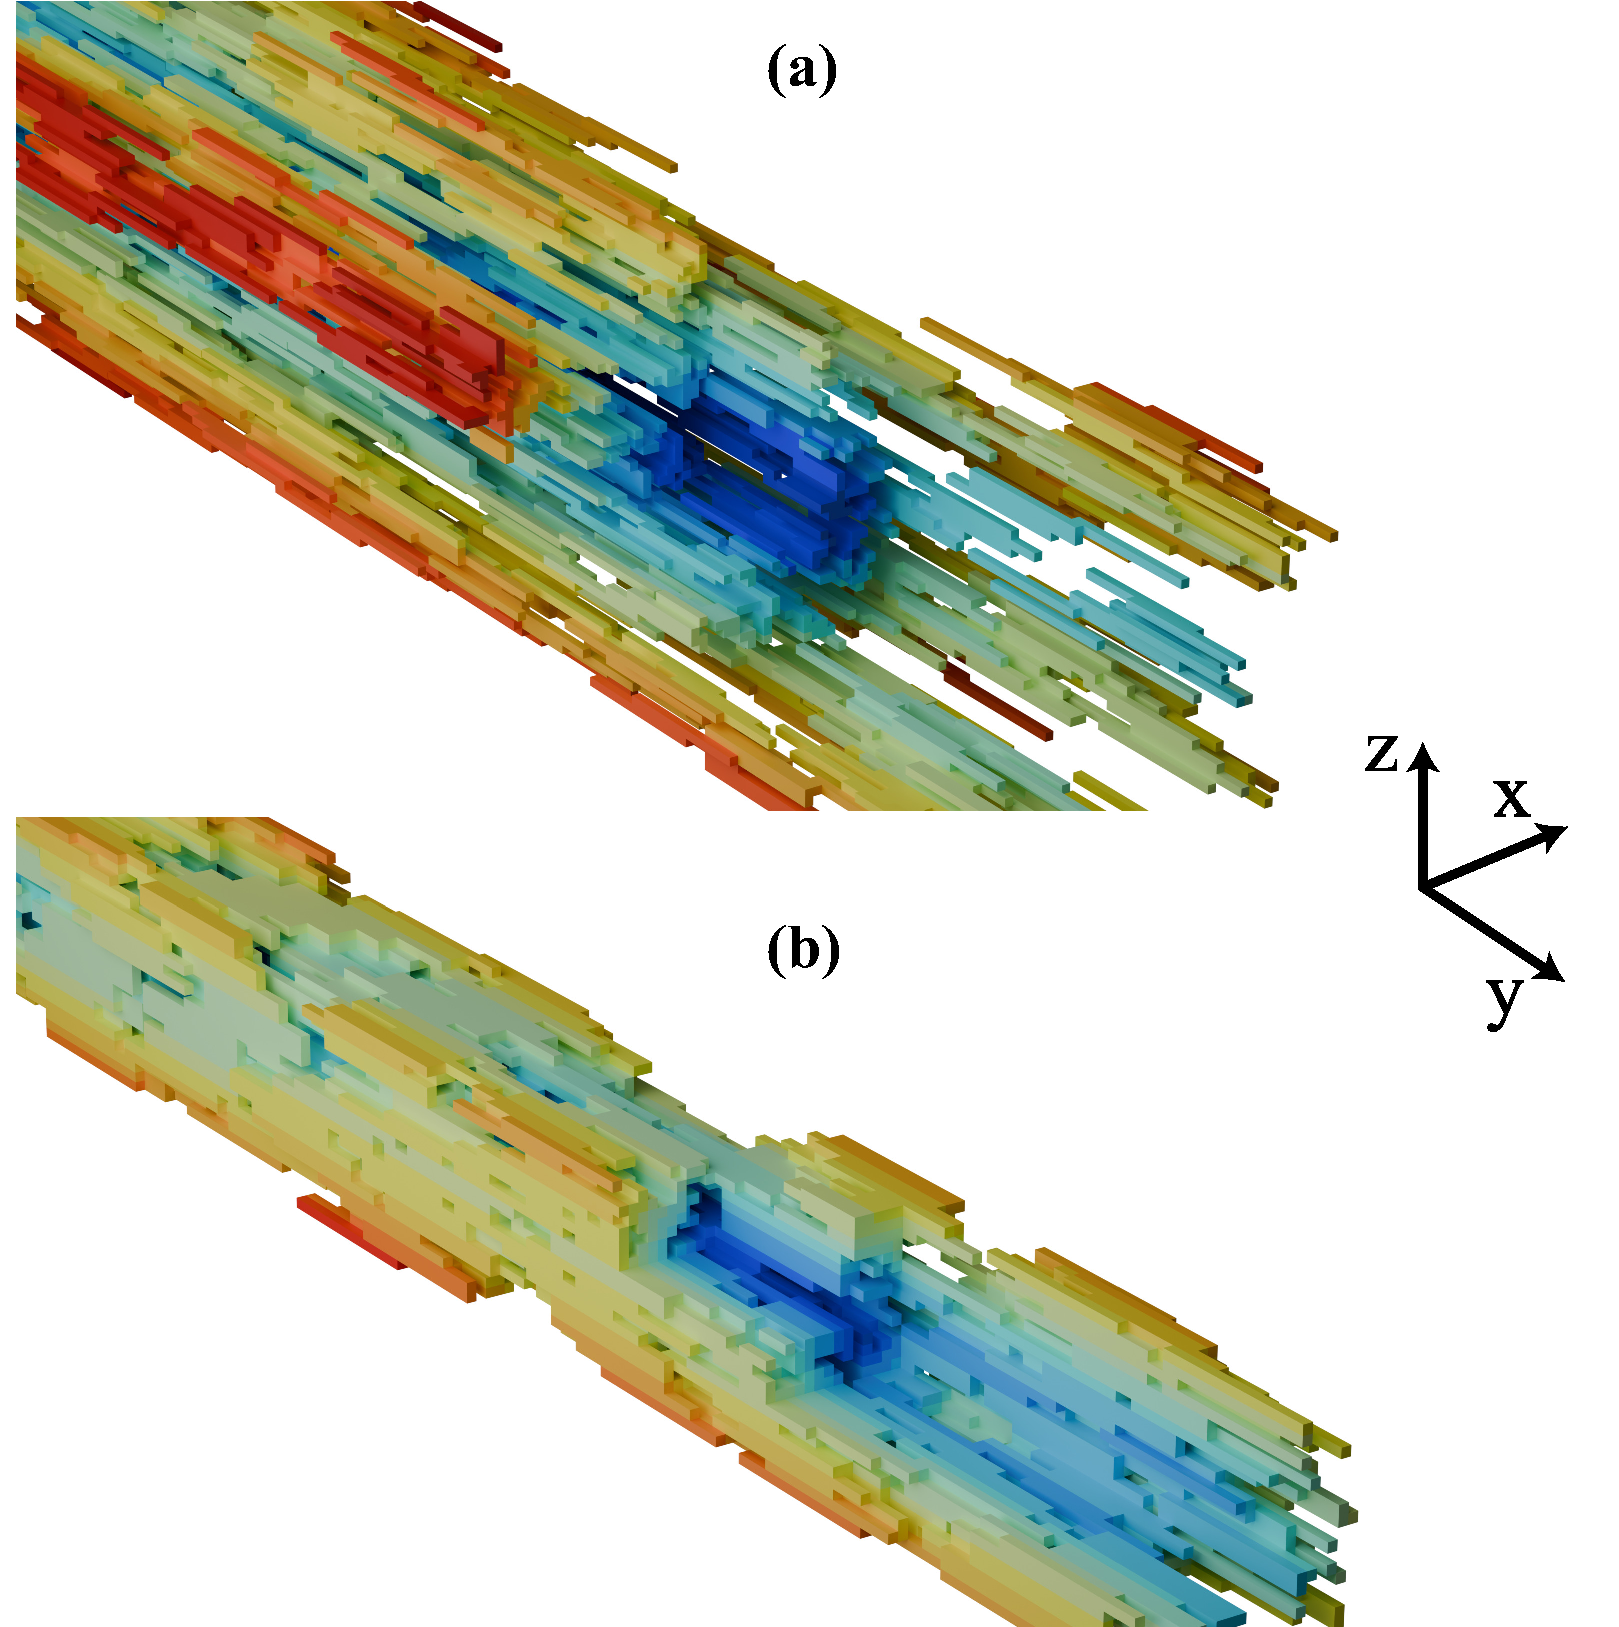
\includegraphics[width=0.7\textwidth]{figure_1.pdf}
	\caption{Representative fibril segments generated with the DLA algorithm containing 30,000 molecules. Panels $(a)$ and $(b)$ show typical fibrils obtained with $T_s = 2$ (short-term diffusion) and $T_s = 8192$ (long-term diffusion), respectively. Colors indicate the relative time of attachment, from early (blue) to late (red).}
	\label{fig_1}
\end{figure}


The generated fibrils exhibit complex, heterogeneous packing with internal voids whose prevalence depends strongly on $T_s$ (Fig.~\ref{fig_1}), which represents the number of diffusion attempts a molecule undergoes to minimize the external surface area and fill internal gaps. For $T_s = 2$, the fibril displays an open architecture characterized by large, visible gaps between molecular clusters. For intermediate values of $T_{s}$, the structure undergoes a progressive compaction as molecules more effectively find optimal sites to fill internal voids. Consequently, for $T_s = 8192$, the fibril becomes substantially more compact and homogeneous, with drastically reduced void space.


Although fibril growth proceeds primarily along the longitudinal axis ($y$-direction), the influence of the surface diffusion parameter $T_s$ is most pronounced in the radial organization of the structure ($x$-$z$ plane), as illustrated in Fig.~\ref{fig_2}. At low $T_s$ , the projected cross-sections are open and branched. As $T_s$ increases, however, the packing becomes progressively more compact and regular, reaching a highly uniform configuration at $T_s = 8192$. Since a higher local packing density implies a greater number of intermolecular contacts, this morphological transition suggests that fibrils formed at larger $T_s$ exhibit enhanced connectivity and mechanical stability \cite{Mohammadkhah2023}.

\begin{figure}[!htb]
	\centering
	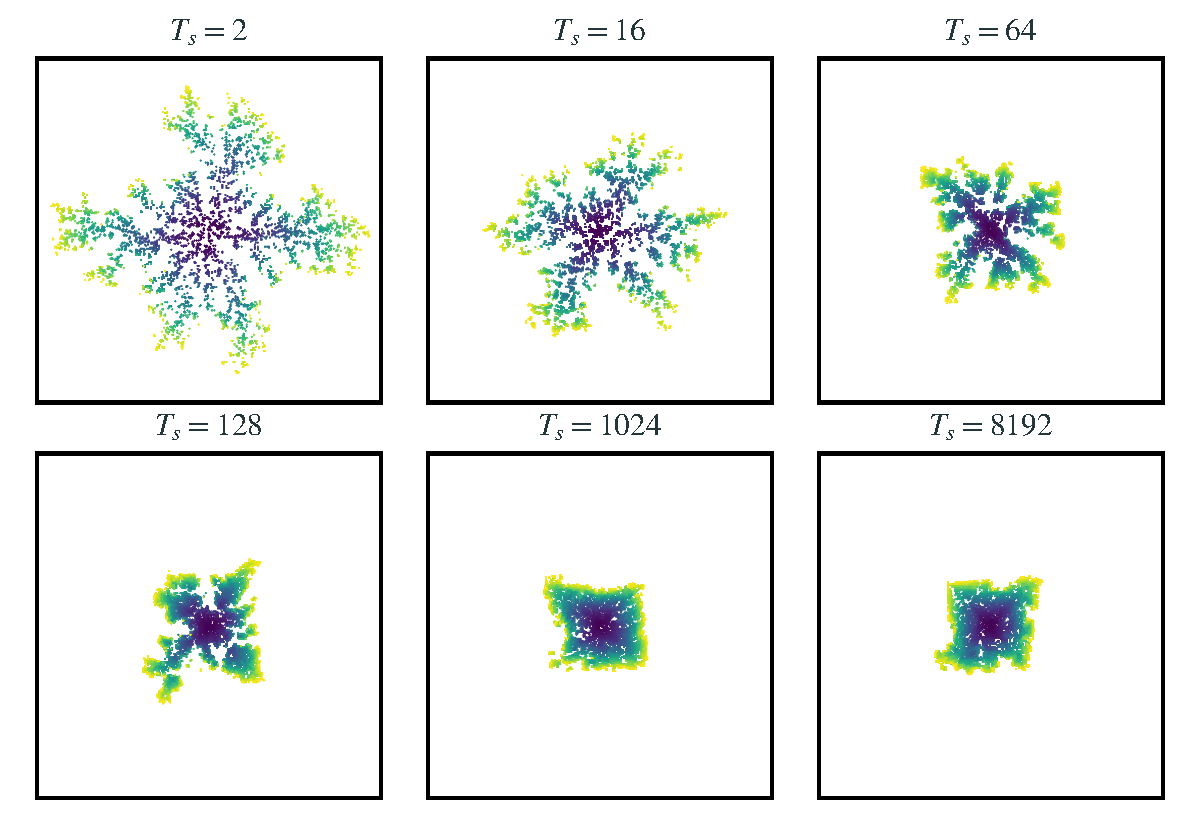
\includegraphics[width=1.\textwidth]{figure_2.pdf}
	\caption{Representative projected central segments ($x$-$z$ plane) for $T_s = 2, 16, 64, 128, 1024,$ and $8192$. Increasing $T_s$ illustrates a clear transition from a sparse, irregular morphology at low values to dense, radially symmetric packing at high values. The color gradient (blue to yellow) indicates the temporal sequence of molecular incorporation, from early-attached to recently added molecules.}
	\label{fig_2}
\end{figure}

To quantify how $T_s$ modulates fibril structure, we first estimated the fractal dimension of the central segment, defined as the region extending from $y=-100$ to $y=100$. For each $T_s$, we generated $50$ fibrils and isolated this central region from each. Within each central segment, we extracted $11$ cross-sections at intervals of $18~\text{l.u.}$ between $y=-90$ and $y=90$, yielding a total of $550$ cross-sections per $T_s$ value. For each cross-section, we computed the center of mass and the maximum radius enclosing all particles (segments of molecules); $R_{\text{max}}$ was subsequently defined as the largest of these $550$ radii. The mass $m(R)$ was measured as the number of particles within a circular region of radius $R$ centered at the cross-section's center of mass. For each value of $R$ spanning from $R_{\text{min}} = 5~\text{l.u.}$ to $R_{\text{max}}$, we computed the mean mass $\langle m(R) \rangle$ by averaging over all $550$ cross-sections \cite{Vicsek1991}. The fractal dimension $D_f$ was then estimated from the mass--radius scaling relation \cite{Giordano2012,stauffer2018introduction}:

\begin{equation}
	\langle m(R) \rangle \sim R^{D_{f}},
	\label{eq1}
\end{equation}
by performing a linear fit on a log-log plot of $\langle m(R) \rangle$ versus $R$.

As shown in Fig.~\ref{fig_3}, $D_f$ depends strongly on $T_s$, providing a quantitative measure of the morphological transition observed in Fig.~\ref{fig_2}. For $T_s = 2$, we find that $D_f = 1.708 \pm 0.005$, close to the characteristic value of two-dimensional diffusion-limited aggregation ($D_f \approx 1.71$) \cite{Witten1983}. As $T_s$ increases, $D_f$ rises and saturates at $D_f = 1.963 \pm 0.001$ for $T_s = 8192$, approaching the Euclidean limit of $D_f = 2.0$ expected for a compact two-dimensional disk. Thus, increasing post-attachment mobility drives a crossover from diffusion-limited, fractal packing to nearly space-filling cross-sections. 


\begin{figure}[h!]
	\centering
	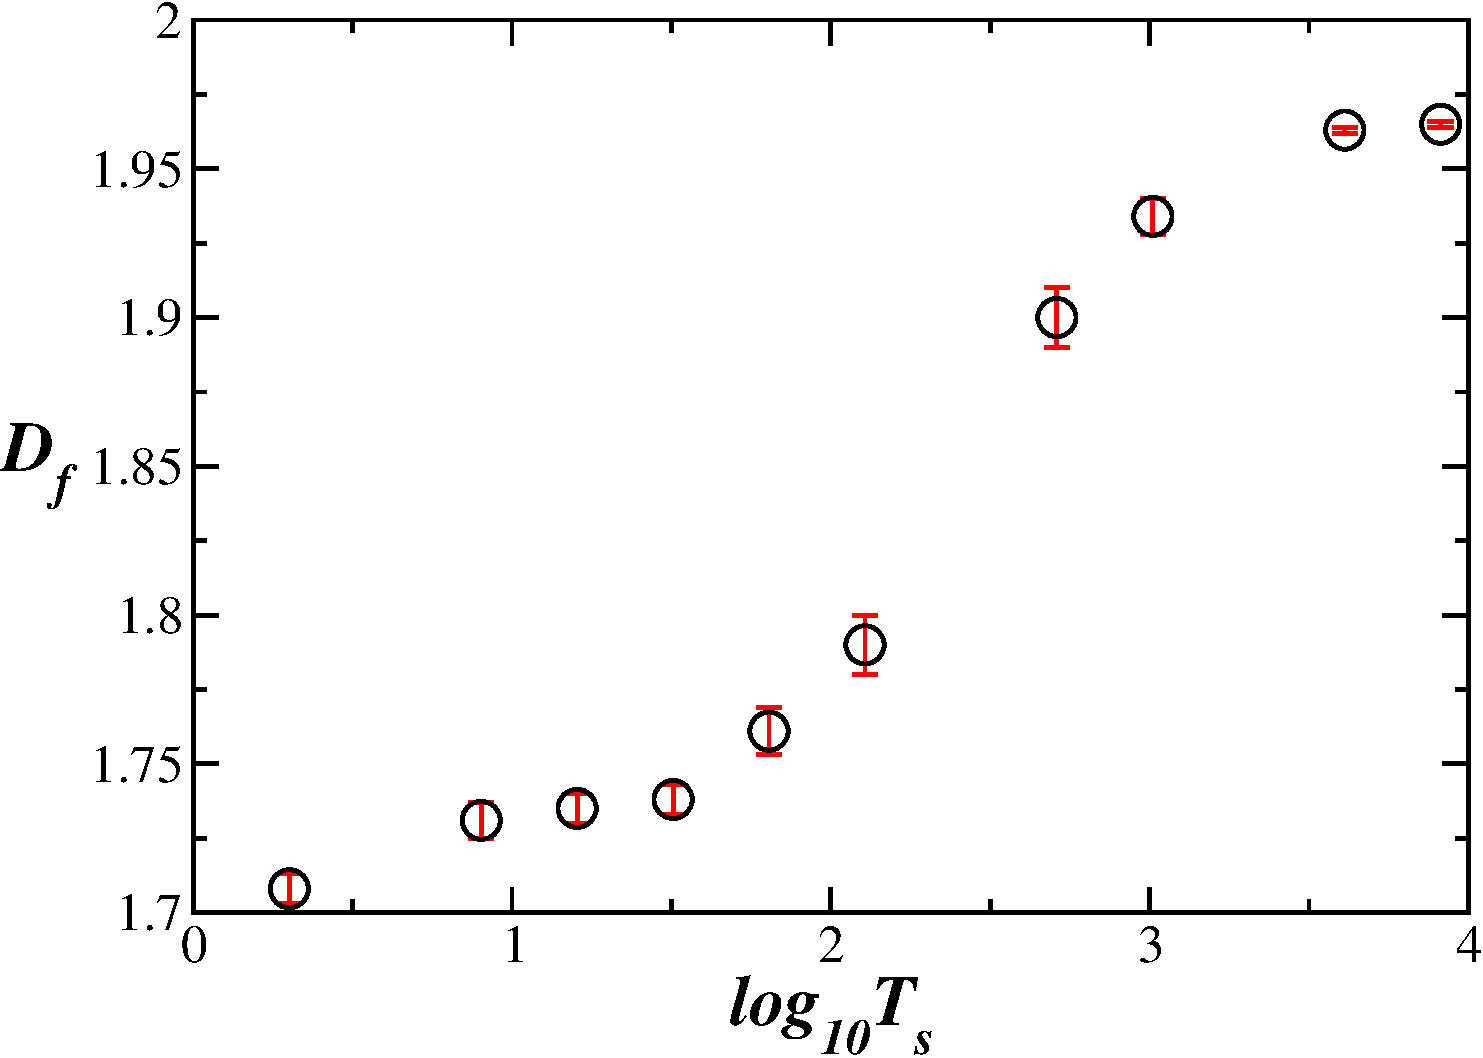
\includegraphics[width=0.7\textwidth]{figure_3.pdf}
	\caption{Average fractal dimension $D_f$ as a function of the diffusion parameter $T_s$ on a log-linear plot. Error bars are shown in red. The fractal dimension increases from $D_f = 1.708 \pm 0.005$ at $T_s = 2$ to $D_f = 1.963 \pm 0.001$ for $T_s = 8192$.}
	\label{fig_3}
\end{figure}		


\subsection{Mechanical Model for Fibril Rupture}

To connect the $T_s$-dependent fibril architecture to mechanical failure, we modeled rupture using a progressive, probabilistic fracture framework commonly employed for disordered networks \cite{z2019,Gilabert1987,Noguchi2024}. Because collagen molecules are represented as rigid rods that do not undergo continuous deformation prior to failure, we do not attempt to resolve deterministic crack propagation. Instead, intermolecular bonds fail stochastically under an applied axial force, and whole molecules detach from the load-bearing network with a stress-dependent probability. The procedure consists of:
$(i)$ isolating a trunk (force-carrying core) with dimensions $S_x = 17$, $S_y = 201$, and $S_z = 17$ l.u. \cite{Parkinson1997}. Truncation inevitably creates disconnected dangling ends that do not contribute to force transmission \cite{Herrmann1984}; we therefore
$(ii)$ identify the backbone (active skeleton) within the trunk prior to applying tensile loading \cite{Moreira2012}.

Backbone extraction proceeds in two passes. In the first pass, molecules at $y = 1$ are marked as active, and we scan upward to $y = S_y$, progressively marking molecules in contact with active ones; unmarked molecules are then removed. In the second pass, molecules at $y = S_y$ are marked as active, and we scan downward to $y = 1$ using the same connectivity rule; only molecules marked active after this pass are retained, defining the final backbone \cite{Parkinson1997} (Fig.~\ref{fig_4}).

\begin{figure}[h!]
	\centering
	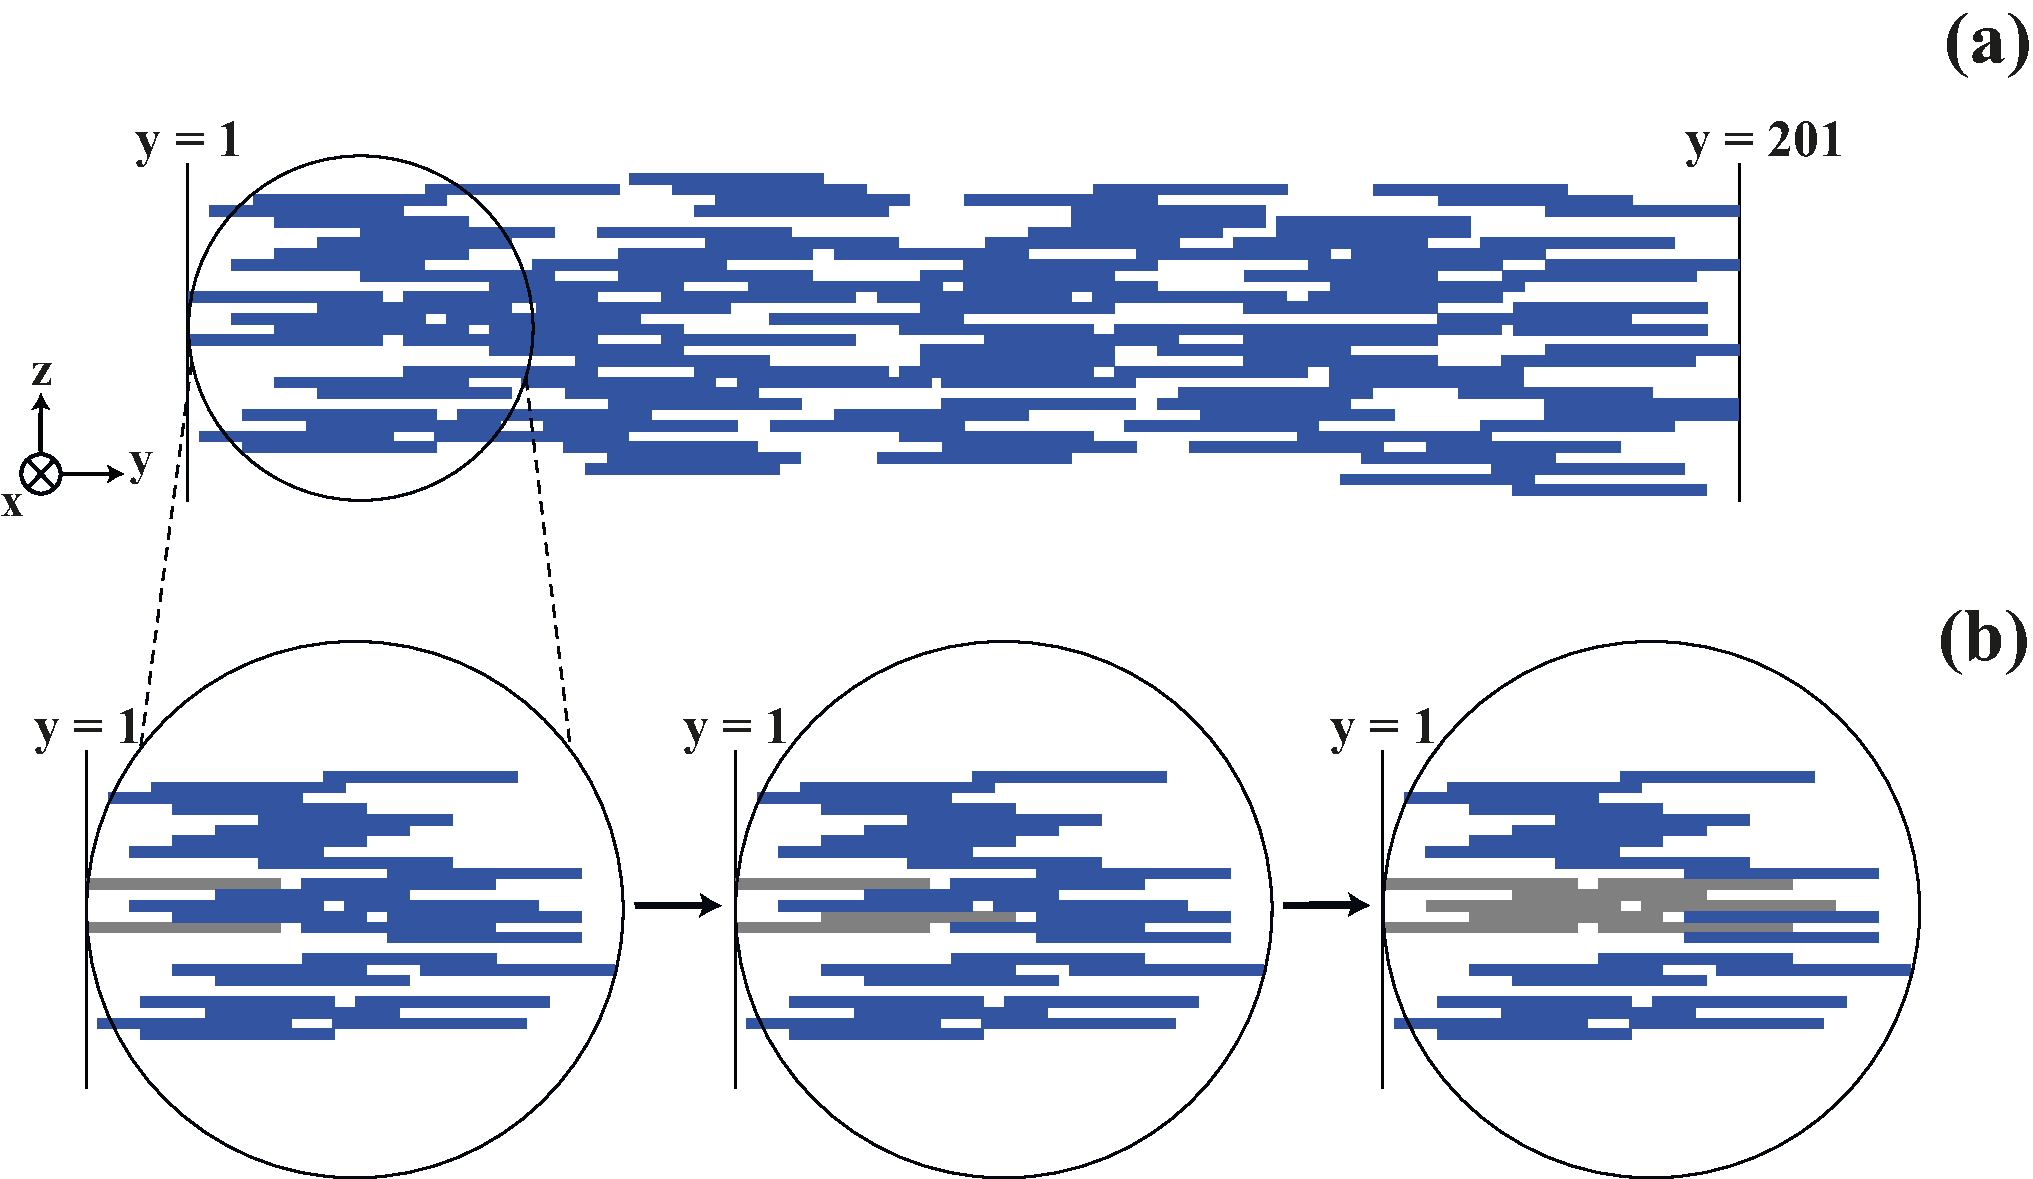
\includegraphics[width=\textwidth]{figure_4.pdf}
	\caption{(a) Two-dimensional visualization of an isolated fibril trunk used to extract the backbone. The circle highlights the region where the identification procedure starts ($y = 1$). (b) Example of the backbone identification procedure from left to right: molecules marked as active are highlighted in gray as connectivity is propagated along the trunk, yielding the final backbone.}
	\label{fig_4}
\end{figure}

With the backbone identified, we simulate the effects of axial tension along the fibril's axis ($y$) by progressively increasing a dimensionless force parameter $F$, where $F$ regulates the removal of molecules in a probabilistic fashion. At each cross-section $i$, we define the effective load-bearing area as the number of backbone segments intersecting that plane, $N(i)$. Each discrete segment is assigned a unit area on the lattice \cite{Parkinson1995}; assuming uniform load sharing, the local tensile stress at cross-section $i$ is:

\begin{equation}
	\sigma(i) = \dfrac{F}{N(i)}.
	\label{eq2}
\end{equation}

We assume that local failure occurs by rupturing intermolecular bonds so that molecules detach from each other rather than break \cite{Parkinson1997}. For a molecule spanning $n$ cross-sections, the mean stress is computed as the average of the local cross-sectional stresses:

\begin{equation}
	\sigma_{M} = \dfrac{1}{n}\sum_{i=1}^{n} \sigma(i).
	\label{eq3}
\end{equation}

A molecule's resistance to detach is assumed to scale with the number of intermolecular contacts it forms within the backbone \cite{Vater1979}. For each molecule, we count first-neighbor contacts for every segment in each intersected cross-section and sum these contributions to obtain the total coordination number $K$. The corresponding failure threshold is $\sigma^{\mathrm{th}} = K\sigma_c X$, where $X$ is a quenched strength variable drawn once per molecule before loading (Eq.~\ref{eq4}) and $\sigma_c$ is the critical stress for bond rupture; we set $\sigma_c = 1$, assuming identical molecules. To simplify the model, both the applied force parameter $F$ and the critical stress $\sigma_c$ are treated as dimensionless quantities in arbitrary units. Hence, $\sigma_c = 1$ represents the normalized threshold for intermolecular bond rupture, which allows us to focus on relative mechanical behavior rather than absolute physical values.

The strength of each molecule is fixed before loading rather than resampled during it. Molecule $i$ draws a variable $X_i \in [0,1]$ once, with cumulative distribution

\begin{equation}
	P(X_i \le x) = x^{m}, \qquad \sigma^{\mathrm{th}}_{i} = K_i \sigma_c X_i,
	\label{eq4}
\end{equation}
and fails when its mean stress $\sigma_{M,i}$ exceeds its threshold $\sigma^{\mathrm{th}}_{i}$. Under this rule the probability that a molecule of coordination $K$ has failed once its mean stress reaches $\sigma$ is $(\sigma/K\sigma_c)^{m}$, so Eq.~(\ref{eq4}) is the original removal probability of our model read as a distribution of strengths; the weakening of a molecule as it loses neighbors, through $K$, is preserved unchanged. Here $m$ is the Weibull modulus, a dimensionless shape parameter controlling the scatter of the strengths~\cite{Parkinson1997,Jones2012}: larger $m$ yields a narrower distribution of rupture strengths, smaller $m$ a broader one. No Weibull modulus has been reported for single collagen fibrils, so we sweep $m \in \{1,2,3,5,10\}$ and retain $m = 2$, the value used by Parkinson et al.~\cite{Parkinson1997}, as the illustrative case in the figures. Fig.~\ref{fig_5} schematically illustrates the calculation of $\sigma(i)$, $\sigma_{M}$, and $K$ for a representative molecule.

Equations~(\ref{eq2})--(\ref{eq4}) combine uniform load sharing within each cross-section with local, coordination-dependent molecular resistance. When a molecule is removed, $N(i)$ decreases only in the cross-sections it previously occupied, and the corresponding stress increase is shared uniformly among the remaining segments within each affected cross-section. The removal also reduces $K$ for the molecule's nearest neighbors, lowering their failure thresholds. Together these define a hybrid load-transfer mechanism: stress equilibrates uniformly among the active segments of each cross-section, while the failure thresholds respond to local coordination. Two features of the construction set it apart from the idealized limits. Stress is redistributed without any distance-dependent elastic kernel, so the coordination channel carries the only local information; and $N(i)$ varies along the fibril while molecules span different sets of cross-sections, so no single globally shared stress governs the bundle. The model therefore combines features of equal and local load sharing without mapping onto either limit.

\begin{figure}[ht!]
	\centering
	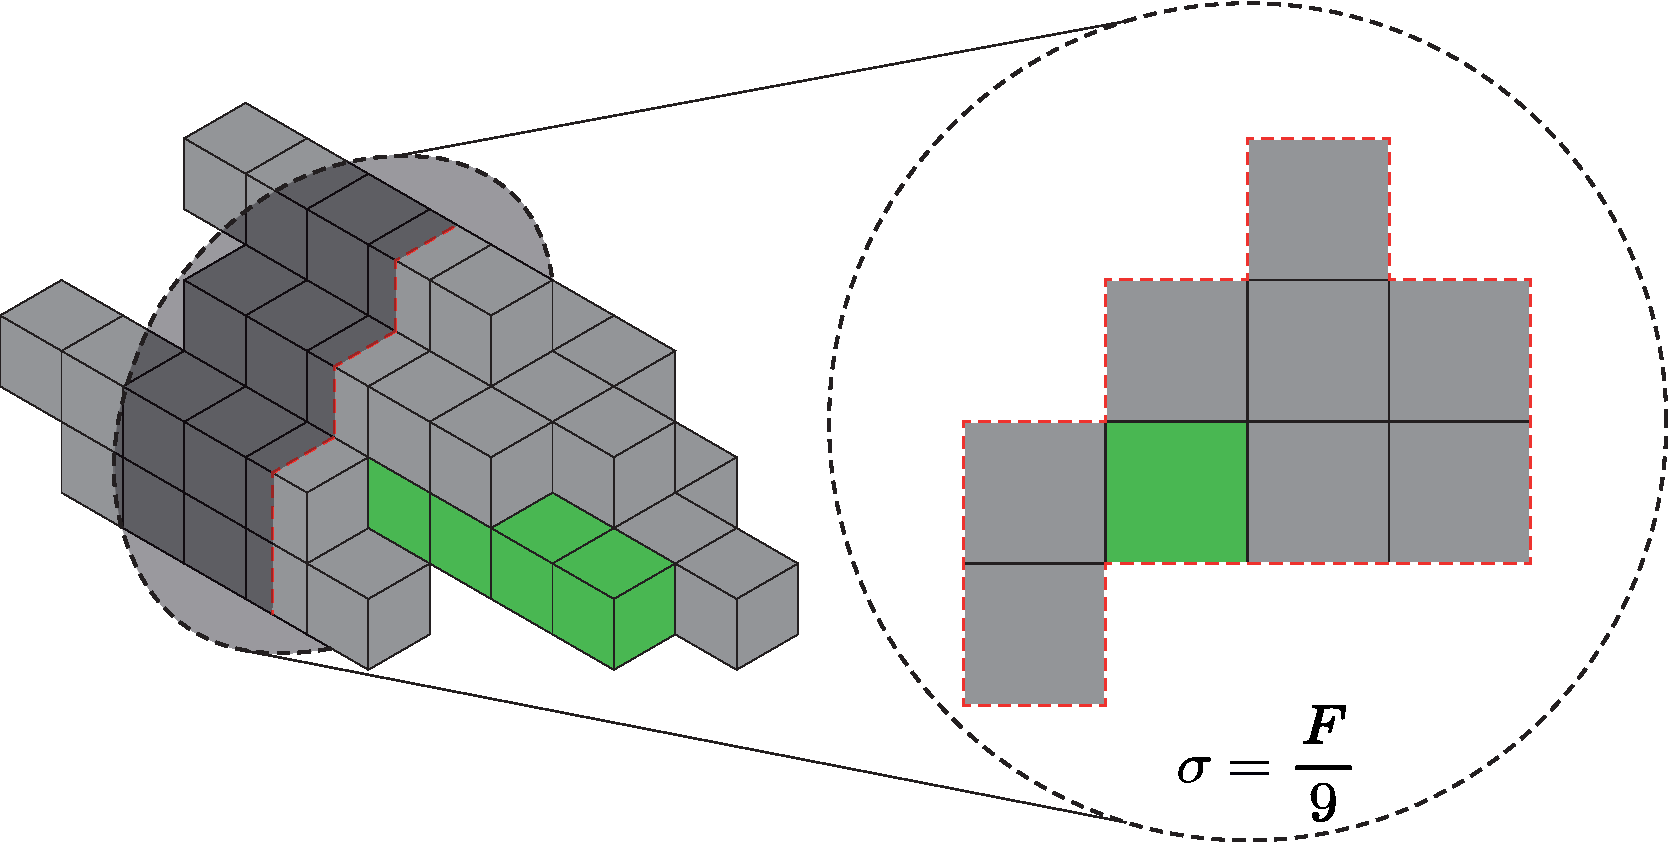
\includegraphics[width=0.9\textwidth]{figure_5.pdf}
	\caption{Schematic illustration of the computation of the removal probability $P_{R}$ for a representative molecule (green). Left: a portion of the backbone where each rectangle represents a molecule (drawn with five segments for clarity). The green molecule intersects multiple cross-sections; for each intersected cross-section $i$, the local stress is $\sigma(i)=F/N(i)$ (right; example with $N(i)=9$, giving $\sigma(i)=F/9$).}
	\label{fig_5}
\end{figure}

Because $\sigma_{M,i} = F a_i$, with $a_i = \langle 1/N(i) \rangle$ averaged over the cross-sections that molecule $i$ spans, every molecule has a well-defined failure threshold $F^{*}_{i} = K_i \sigma_c X_i / a_i$. The loading is strictly quasi-static and extremal, ensuring that the entire rupture process proceeds through a sequence of equilibrium states. The external force is raised continuously until it reaches the smallest $F^{*}_{i}$ present in the current configuration. At this fixed force, the corresponding molecule fails; stresses and coordinations are then recomputed, and molecules disconnected from both ends are removed. This iterative update continues at constant force until no remaining molecule exceeds its failure threshold under the updated stress distribution across the fibril. Only after the system fully relaxes into a stable configuration—where every surviving molecule satisfies $F^{*}_{i} > F$—is the external force incremented again. Rupture is defined as the appearance of a completely void cross-section, signaling failure of the backbone. The steps of this process are schematized in Fig.~\ref{fig_6}.

To capture the statistical nature of this failure process and account for the inherent disorder in molecular strengths, we systematically sampled both the fibril architecture and the strength distribution. Specifically, for each condition of $T_s$ and $m$, we analyzed an ensemble of $200$ distinct fibrils ($3\times 10^4$ molecules each) subjected to $50$ independent rupture realizations, yielding $10^4$ realizations per $(T_s, m)$ combination. Realizations of the same fibril differ solely in the assigned random strengths. Throughout each simulation, we monitored the progress of damage by recording the molecules evicted in every cascade along with the precise external force at which failure occurred.

\begin{figure}[ht!]
	\centering
	\includegraphics[width=0.9\textwidth]{figure_6.pdf}
	\caption{Schematic view of the load-bearing backbone and the stages of the rupture process. (a) Two-dimensional view of the backbone subjected to an axial force $F$ along the $y$-axis. Each molecule (gray) carries a failure threshold $\sigma^{\mathrm{th}} = K\sigma_c X$ drawn once before loading (Eq.~\ref{eq4}); the external force is raised to the smallest failure force in the configuration, and the molecule that reaches it fails. (b) Progressive damage after some molecules have been removed, represented by red dashed lines. (c) Rupture occurs when a cross-section becomes completely empty (solid lines), eliminating the continuous load path.}
	\label{fig_6}
\end{figure}

With this extensive dataset, we quantified the overall mechanical resistance of the fibrils by evaluating the backbone rupture force, $F_{\mathrm{r}}$, across the different Weibull moduli $m$. As shown in the main plot of Fig.~\ref{fig_7}, $F_{\mathrm{r}}$ exhibits a qualitatively similar dependence on $T_{\mathrm{s}}$ ($\log_{10} T_{\mathrm{s}}$) regardless of $m$. All curves increase monotonically with $T_{\mathrm{s}}$ before reaching a saturation plateau, $F_{\mathrm{sat}}$, whose magnitude grows with $m$. Fibrils with higher $m$ values are markedly stronger; for instance, at $m = 2$, the mean rupture force increases by an order of magnitude, from $151 \pm 36$ at $T_{\mathrm{s}} = 2$ to $1532 \pm 218$ at $T_{\mathrm{s}} = 8192$. Notably, $83\%$ of this total strength gain is already achieved by $T_{\mathrm{s}} = 128$, beyond which further increases in $T_{\mathrm{s}}$ yield negligible enhancements in mechanical resistance. The right inset demonstrates a universal curve collapse when normalizing the rupture force by its saturation value ($F_{\mathrm{r}} / F_{\mathrm{sat}}$ versus $\log_{10} T_{\mathrm{s}}$), confirming a scale-invariant behavior independent of $m$. Finally, the left inset shows that the saturation force $F_{\mathrm{sat}}$ grows asymptotically with $m$, following an exponential dependence accurately fitted by $F_{\mathrm{sat}} = a(1 - e^{-m/b})$. 


\begin{figure}[ht!]
	\centering
	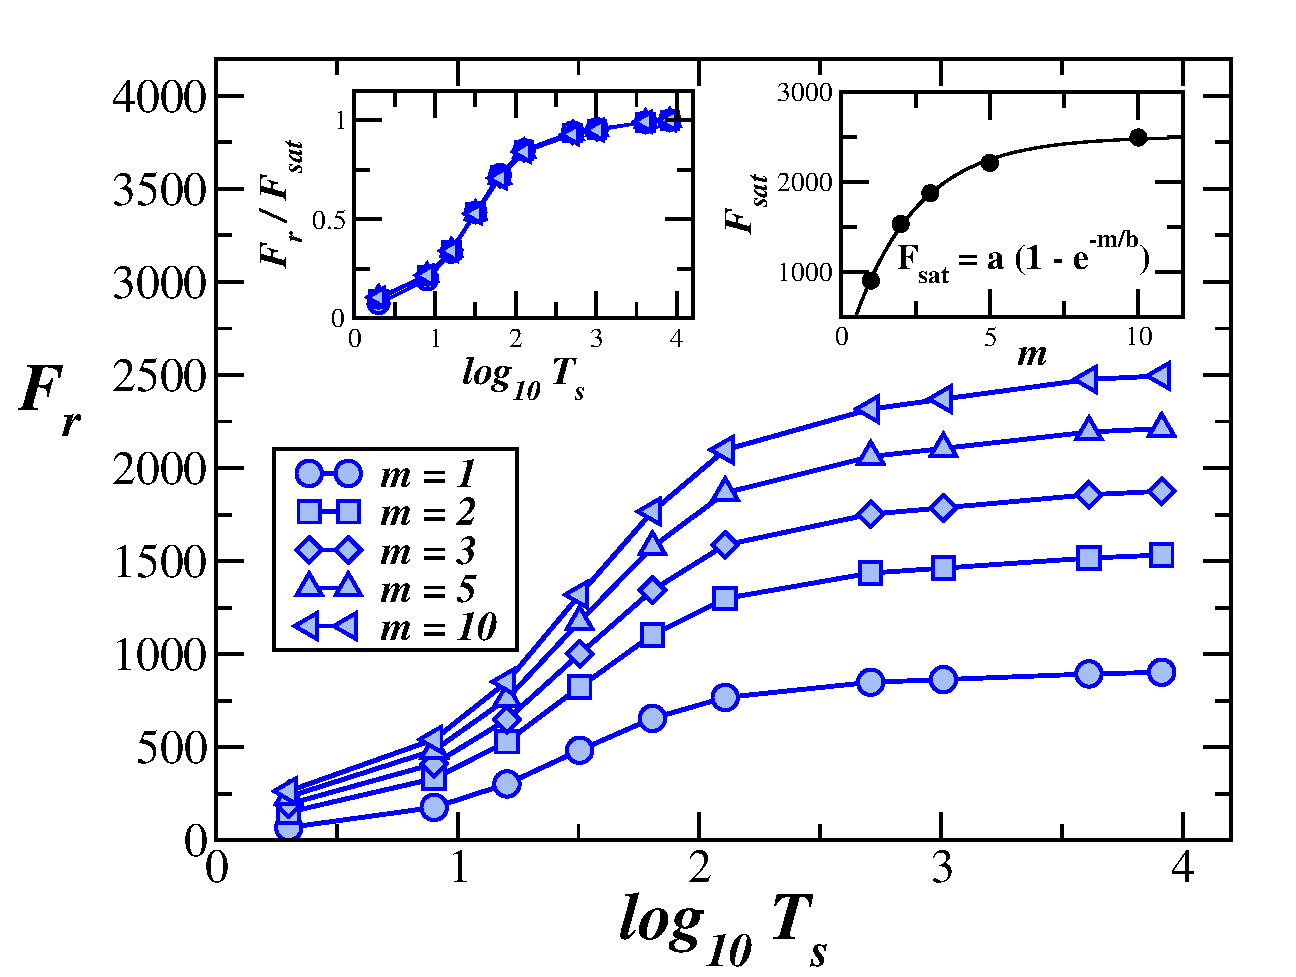
\includegraphics[width=\textwidth]{figure_7.pdf}
	\caption{ Mean rupture force $F_{\mathrm{r}}$ as a function of $T_{\mathrm{s}}$ for five values of the Weibull modulus $m$. The right inset shows the curve collapse of $F_{\mathrm{r}}/F_{\mathrm{sat}}$ versus $T_{\mathrm{s}}$, where $F_{\mathrm{sat}}$ corresponds to the saturation value of $F_{\mathrm{r}}$ at high $T_{\mathrm{s}}$ values, confirming a universal behavior across different values of $m$. The left inset shows how $F_{\mathrm{sat}}$ behaves as a function of $m$, where the solid line represents the fit $F_{\mathrm{sat}} = a(1 - e^{-m/b})$ with $a = [\text{value}]$ and $b = [\text{value}]$.}
	\label{fig_7}
\end{figure}


While these macro-level findings establish that $F_{\mathrm{r}}$ grows systematically with $T_{\mathrm{s}}$, the global fractal dimension $D_f$ alone—a single static value characterizing the average cross-sectional morphology at assembly—cannot fully capture the underlying failure dynamics. To bridge this global morphological characterization with the local mechanics of rupture, we now track two time-resolved structural quantities: the mean load-bearing cross-sectional count $\langle N \rangle$ and the mean coordination number $\langle K \rangle$, both normalized by their initial pre-loading values $\langle N_0 \rangle$ and $\langle K_0 \rangle$. Unlike $D_f$, these are inherently dynamical quantities that evolve as molecules are progressively evicted from the backbone under increasing external force $F$. Together, they directly govern the local failure threshold of each individual molecule via $F_i^* = K_i \sigma_c X_i / a_i$ (Eq.~\ref{eq4}), where $a_i \propto 1/N$. Figure~\ref{fig_8} illustrates the dynamic evolution of both quantities across six representative values of $T_{\mathrm{s}}$ at $m = 2$.

The coordination number Fig.~\ref{fig_8}a decreases monotonically for all architectures. As each molecule fails and is detached, its nearest neighbors lose lateral contacts and their coordination $K$ drops accordingly. The force at which each curve terminates identifies the rupture event and grows systematically with $T_s$, consistent with Fig.~\ref{fig_7}. More strikingly, the fraction of coordination retained at the moment of rupture is strongly architecture-dependent: $T_s = 2$ loses approximately $20\%$ of $\langle K_0 \rangle$ before failing at $F \approx 200$, whereas $T_s = 128$ retains more than $97\%$ of its initial coordination all the way to $F \approx 1600$. Compact fibrils are therefore not only stronger in absolute terms but also far more resilient at the level of molecular connectivity — their lateral contact network degrades much more slowly per unit of applied force. Since $K$ directly sets the failure threshold via (Eq.~\ref{eq4}), this sustained coordination keeps individual thresholds high throughout loading and prevents the runaway weakening that drives early failure in open architectures.

\begin{figure}[ht!]
	\centering
	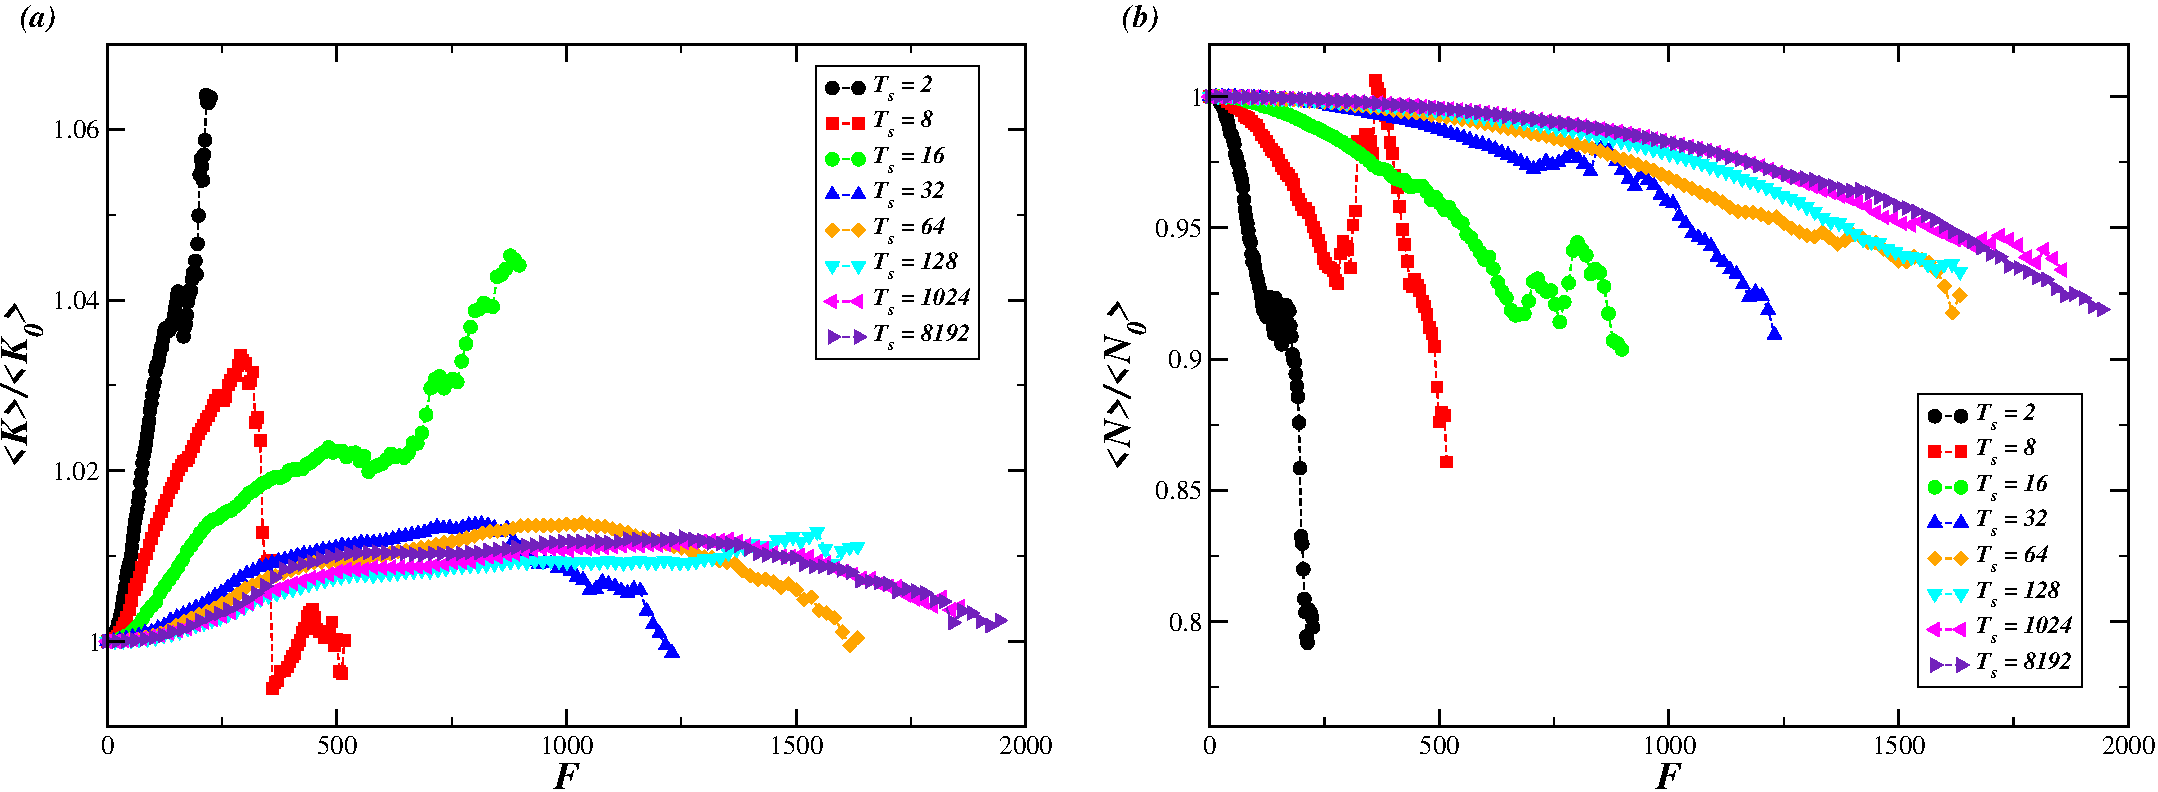
\includegraphics[width=\textwidth]{figure_8.pdf}
	\caption{Evolution of the normalized mean coordination number $\langle K \rangle / \langle K_0 \rangle$ (a) and normalized mean load-bearing cross-sectional count $\langle N \rangle / \langle N_0 \rangle$ (b) as functions of the applied force $F$, for $T_s = 2, 8, 16, 32, 64$, and $128$ at Weibull modulus $m = 2$. Quantities are normalized by their respective values immediately before loading, $\langle K_0 \rangle$ and $\langle N_0 \rangle$, and averaged over the ensemble of backbone realizations. Each curve terminates at the mean rupture force $F_\text{r}$ of the corresponding architecture. }
	\label{fig_8}
\end{figure}

The mean load-bearing area Fig.~\ref{fig_8}b displays a non-monotonic behavior whose character changes markedly with $T_{\mathrm{s}}$, directly mirroring the morphological transition quantified by $D_f$. For open fibrils ($T_{\mathrm{s}} = 2$ and $8$), $\langle N \rangle / \langle N_0 \rangle$ rises steeply and irregularly from the onset of loading, reaching peaks of approximately $+6.5\%$ and $+3.5\%$ above $\langle N_0 \rangle$, respectively, before falling toward rupture. This initial increase stems from a structural selection effect rooted in the spatial heterogeneity of open architectures (Figs.~\ref{fig_1} and \ref{fig_2}): molecules spanning the thinnest cross-sections $N(i)$ experience disproportionately higher local stresses $\sigma(i) = F/N(i)$ and fail preferentially at lower forces. Their early removal eliminates these sparse, high-stress sections from the active backbone, shifting the ensemble average $\langle N \rangle$ upward—acting as an early self-strengthening mechanism where the fibril sheds its weakest cross-sections to leave behind a denser, more load-capable core. The prominent, irregular fluctuations along this rise directly reflect the spatial non-uniformity of the fibril itself. As $F$ continues to grow and this reserve of sparse sections is exhausted, the average turns over and falls toward rupture. The case $T_{\mathrm{s}} = 16$ marks a transitional regime with a broader peak and attenuated fluctuations, consistent with an intermediate fractal dimension $D_f \approx 1.74$ (Fig.~\ref{fig_3}). In contrast, for compact fibrils ($T_{\mathrm{s}} \ge 32$), where the fractal dimension $D_f$ shows a significant shift toward the Euclidean limit ($D_f \to 2.0$), the cross-sectional packing becomes nearly uniform. This narrow distribution of $N(i)$ leaves little variance for selective pruning: the large fluctuations disappear, and $\langle N \rangle / \langle N_0 \rangle$ grows smoothly to a mild maximum of only $\approx +1\%$ before declining gently in the terminal approach to failure. The smoothness of $\langle N \rangle / \langle N_0 \rangle$ for $T_{\mathrm{s}} \geq 32$ is thus a direct dynamical signature of structural homogeneity, driven by the same compaction mechanism responsible for the saturation of $F_{\mathrm{r}}$ observed in Fig.~\ref{fig_7}.  


The joint behavior of $\langle K \rangle(F)$ and $\langle N \rangle(F)$ thus provides a coherent microscopic account of the $T_s$ dependence reported before. Compact fibrils enter the loading protocol with larger $\langle N_0 \rangle$ and $\langle K_0 \rangle$ — a direct consequence of their higher $D_f$ — and both quantities degrade more slowly as $F$ increases. Since $N$ controls the local stress and $K$ controls the failure threshold, the two channels reinforce each other: a larger $N$ lowers $\sigma = F/N$, and a larger $K$ raises $\sigma^\text{th} = K\sigma_c X$. Compact fibrils benefit simultaneously from both effects throughout the entire loading history, which is the microscopic origin of the order-of-magnitude gain in rupture force between $T_s = 2$ and $T_s = 8192$. The saturation of $F_\text{r}$ visible in Fig.~\ref{fig_7} for $T_s \gtrsim 128$ mirrors the saturation of $N_0$ and $K_0$ as $D_f$ asymptotically approaches the Euclidean limit: once the cross-section is nearly space-filling, further increases in $T_s$ yield diminishing returns in both morphology and mechanical resistance.

%%%%%%%%%%%%%%%%%%%%%%%%%%%%%%%%

During rupture, molecules fail in cascades at constant external force. We define the avalanche as the complete cascade released by one increase of the force: the molecules whose thresholds are exceeded, together with those that lose their continuous load path as a consequence, all removed before the force is raised again. This is the set of molecules that fail between two consecutive increases of the external force, and it is the standard avalanche of fiber-bundle models, a form of crackling dynamics in driven disordered systems \cite{Jaeger1992,Godano1993,Beggs2003,Baraba1996,Alencar2001,Suki1994}. 

We analyze this collective failure process through the framework of avalanche statistics in driven disordered systems~\cite{Zapperi1997a,Zapperi1999,Zapperi1997b}. Here, the avalanche size $s$ corresponds to the number of molecules evicted in a single cascade, as defined above. Figure~\ref{fig_9} displays the pre-terminal cascade size distribution $P(s)$ on logarithmic axes for $T_{\mathrm{s}} = 2, 8, 16$, and $128$ at $m = 2$. Across all conditions, $P(s)$ exhibits a power-law regime over intermediate cascade sizes, followed by a rapid, stretched-exponential cutoff at large $s$. Similar scaling behaviors followed by sharp cutoffs have been documented in numerical studies of impact fragmentation and structural breakdown~\cite{Meibom1996,Diehl2000,Diehl2002,Araujo2003}. Based on these features, $P(s)$ obeys the scaling ansatz:
\begin{equation}
P(s) \propto s^{-\gamma} \exp\left[-\left(\frac{s}{s_c}\right)^\eta\right]
\label{scaling}
\end{equation}
where $\gamma$ is the power-law scaling exponent, while $s_c$ and $\eta$ represent the characteristic cutoff size and stretching exponent, respectively. The solid lines in Fig.~\ref{fig_9} show the best non-linear fits of Eq.~\eqref{scaling} to the data across both the scaling and cutoff regimes for $T_{\mathrm{s}} = 2$ ($\gamma = 2.00 \pm 0.01$, $s_{\mathrm{c}} = 124 \pm 5.67$, $\eta = 3.53 \pm 0.26$) and $T_{\mathrm{s}} = 128$ ($\gamma = 2.55 \pm 0.008$, $s_{\mathrm{c}} = 67 \pm 1.65$, $\eta = 2.71 \pm 0.21$).

A closer examination of $P(s)$ reveals two distinct structural regimes as a function of $T_{{s}}$. At small avalanche sizes  the distributions for all values of $T_{s}$  are nearly indistinguishable, indicating that single- and few-molecule failure events are governed purely by localized threshold dynamics and remain insensitive to the global fibril architecture. In the intermediate-to-large size regime, however, the curves diverge into power-law regimes which depends on the $T_{s}$. For the most open architecture ($T_{\mathrm{s}} = 2$), the distribution follows a shallower decay with $\gamma = 2.00\pm0.013$, signaling a significantly higher probability of large pre-terminal cascades. Conversely, for more compact architectures ($T_{s} \ge 128$), the distributions collapse onto a single, steeper power law with $\gamma = 2.55\pm0.008$, reflecting a systematic suppression of large-scale failure events. Notably, this scaling crossover occurs abruptly between $T_{s} = 2$ and $T_{s} = 128$, directly mirroring the rapid initial rise of the fractal dimension $D_f$ away from the DLA limit (Fig.~\ref{fig_3}). For values above $T_{s}=128$ the exponent  $\gamma$ keep approximately constant within the error bars (data not show) which are in agreement with results for $D_{f}$ , $\langle N\rangle$ and $\langle K\rangle $ that reach a saturation values for $T_{s} \ge 128$ . 
\begin{figure}[ht!]
	\centering
	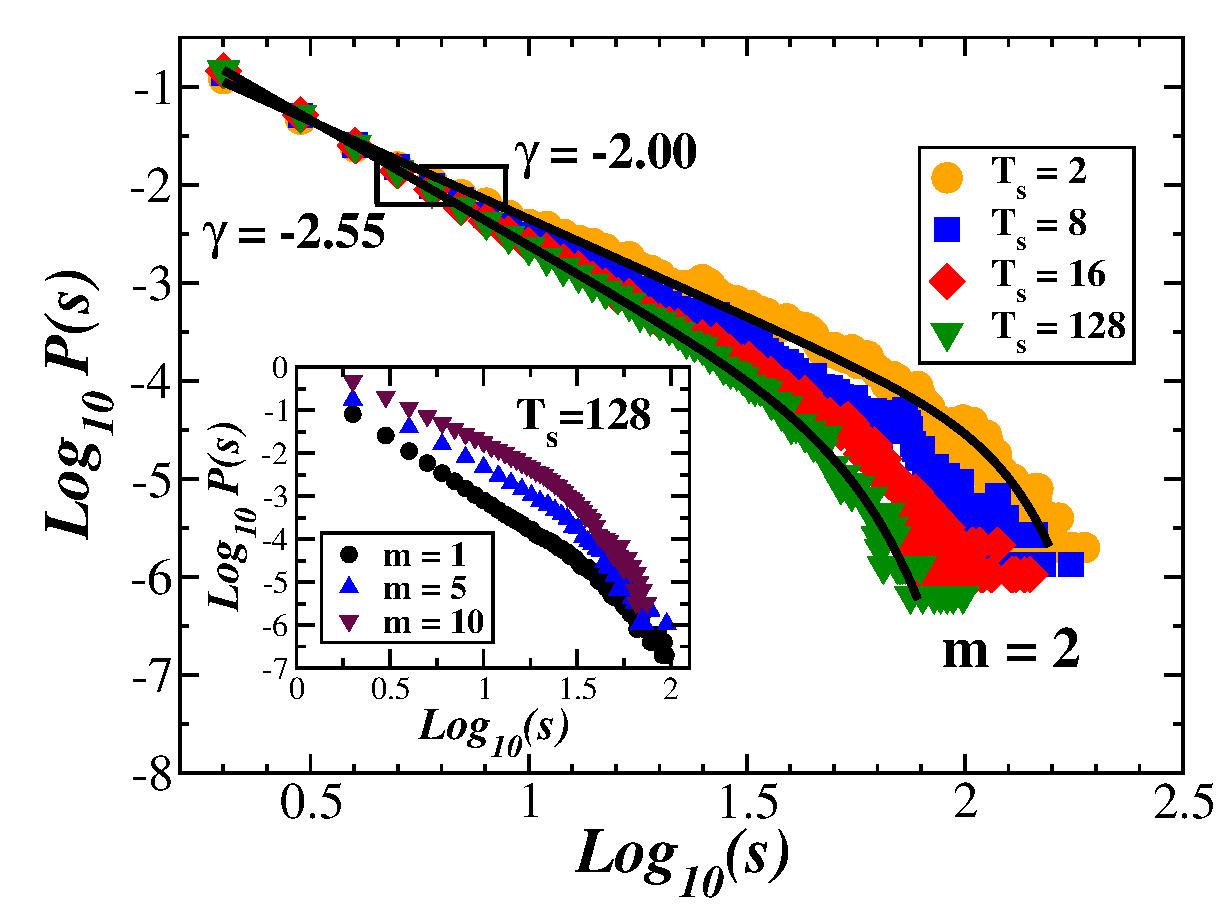
\includegraphics[width=\textwidth]{figure_9.pdf}
	\caption{Avalanche size distribution $P(s)$ on logarithmic axes for $T_s = 2, 8, 16$, and $128$ at Weibull modulus $m = 2$. All curves display a power-law regime followed by a stretched-exponential cutoff. Solid lines are fits of the form
$P(s) \propto s^{-\gamma} \exp\!\left[-\!\left(\frac{s}{s_c}\right)^{\!\eta}\right]$ performed for the cases $T_s = 2$ ($\gamma = 2.00\pm 0.013$, $\eta = 3.53$, $s_c = 124.7$) and $T_s = 128$ ($\gamma = 2.55\pm 0.008$, $\eta = 2.71$, $s_c = 51.61$). Inset: $P(s)$ for $T_s = 128$ and $m = 1, 5$, and $10$. Curves in the inset have been shifted vertically for visual clarity.}
	\label{fig_9}
\end{figure}

This dynamical transition has a clear physical origin rooted in the local structural properties discussed in the previous section. In open fibrils ($T_{\mathrm{s}} = 2, D_f \approx 1.71$), the high spatial heterogeneity gives rise to a broad distribution of cross-sectional counts $N(i)$, as evidenced by the large fluctuations in $\langle N \rangle(F)$ (Fig.\ref{fig_8}b). Molecules in the sparsest cross-sections experience severe local stress concentrations $\sigma(i) = F/N(i)$; upon their failure, the redistributed load readily overloads equally sparse neighboring sections, facilitating cascade propagation. Compounding this effect, the rapid loss of coordination $\langle K \rangle$ observed at $T_{\mathrm{s}} = 2$—a reduction of nearly $20\%$ prior to rupture (Fig.\ref{fig_8}a)—progressively degrades the failure thresholds $F_i^* = K_i \sigma_c X_i / a_i$ of surviving molecules, making them increasingly prone to sequential collapse. Together, the high variance in $N(i)$ and the rapid decay of $K$ sustain extensive cascades, resulting in the shallower exponent $\gamma = 2.00$ and extending the stretched-exponential cutoff up to $s \approx 200$.

For compact fibrils ($T_{s}\ge 32$), both mechanisms are strongly suppressed. The uniform cross-sectional packing associated with $D_f \to 2.0$ leads to a smooth, low-amplitude evolution of $\langle N \rangle(F)$ (Fig.~\ref{fig_8}b) and maintains the coordination number near its initial value $\langle K_0 \rangle$ throughout loading (Fig.~\ref{fig_8}a). This structural homogeneity ensures an even stress distribution and preserves molecular failure thresholds, effectively arresting cascade growth. Consequently, the power-law exponent steepens to $\gamma = 2.55$ and the cutoff shifts to much smaller scales ($s \approx 30\text{--}50$). This sharp reduction confirms that the maximum pre-terminal cascade size is ultimately dictated by the local structural organization of the backbone rather than the total size of the system.

Although our coarse-grained framework adopts necessary physical simplifications—such as representing collagen molecules as rigid rods with a reduced aspect ratio of $18{:}1$~\cite{Parkinson1997,Buehler2008b}, omitting rotational diffusion, and capturing complex biochemical regulation through an effective control parameter $T_{\mathrm{s}}$~\cite{Jiang2004,Yang2009,Kalbitzer2018,Kadler1996,Canty2005,Kadler2008}—these approximations are essential to make the multi-scale physics computationally tractable while retaining its core mechanics. Rather than aiming for exact quantitative metrics or reproducing detailed bond-breaking mechanics~\cite{RuizFranco2022,Provenzano2006,Innocenti2022-lp}, the primary strength and novelty of this model lie in its ability to isolate the fundamental, qualitative relationships between stochastic assembly topology and mechanical resilience. Within this transparent framework, we demonstrate that structural compaction directly strengthens the fibril backbone by modulating the local load-bearing area $N(i)$ and preserving the molecular coordination number $K$, showing that mechanical resilience is achieved without requiring a complex, self-similar load-transfer mechanism.

Importantly, despite these simplifying assumptions, the model's core dynamical prediction—that rupture proceeds via avalanche-like, pre-terminal failure cascades—is strongly supported by experimental evidence. Because avalanche propagation occurs faster than imposed loading rates~\cite{Noguchi2024}, single-molecule force-spectroscopy and tensile tests on individual collagen microfibrils consistently observe discrete force and stress drops resulting from intermolecular cross-link ruptures~\cite{Gutsmann2004,Svensson2013,Deng2024}, directly validating the physical relevance of our cascade framework. By successfully bridging the gap between stochastic fractal assembly and local damage mechanics, this work provides a robust, mechanistic baseline for understanding how geometric packing and spatial heterogeneity govern collective failure in biological tissues, offering valuable insights for both biomechanics and the rational design of resilient, bio-inspired synthetic materials.

\section{Conclusion}
In this work, we coupled a three-dimensional diffusion-limited aggregation model of collagen fibrillogenesis with a progressive probabilistic rupture framework to establish a mechanistic link between assembly kinetics, fibril architecture, and mechanical failure. The post-attachment surface diffusion parameter $T_{\mathrm{s}}$ acts as a single control variable that simultaneously governs morphological organization and fracture resistance. As $T_{\mathrm{s}}$ increases, the fractal dimension $D_f$ rises monotonically from $D_f = 1.708 \pm 0.005$ ($T_{\mathrm{s}}=2$) to $D_f = 1.963 \pm 0.001$ ($T_{\mathrm{s}}=8192$), bridging open fractal assemblies to nearly compact, space-filling architectures. Crucially, $D_f$ sets the pre-loading structural foundation: higher $D_f$ directly yields a larger initial load-bearing area $\langle N_0 \rangle$ and mean coordination number $\langle K_0 \rangle$, granting compact fibrils an immediate mechanical advantage.

During the rupture process, the interplay among $D_f$, $\langle N \rangle$, and $\langle K \rangle$ unveils the microscopic origin of the order-of-magnitude strength gain observed between open and compact architectures. In open fibrils ($T_{\mathrm{s}}=2, D_f \approx 1.71$), severe stress concentration at sparse cross-sections induces early localized failures. While pruning these thinnest sections produces a transient $6.5\%$ self-strengthening rise in $\langle N \rangle / \langle N_0 \rangle$, the rapid $\sim 20\%$ depletion of coordination $\langle K \rangle$ degrades molecular thresholds and sustains extensive cascade propagation ($\gamma = 2.00 \pm 0.013, s_{\mathrm{c}} \approx 124$). Conversely, compact fibrils ($T_{\mathrm{s}} \ge 128, D_f \to 2.0$) feature uniform cross-sectional packing that mitigates stress concentrations, restricts the self-strengthening rise to $\approx 1\%$, and preserves $>97\%$ of $\langle K_0 \rangle$ up to failure. This structural homogeneity suppresses large pre-terminal cascades, steepening the power-law exponent to $\gamma = 2.55 \pm 0.008$ and shifting the cutoff to $s_{\mathrm{c}} \approx 50$.

From a biological and engineering perspective, $D_f$ serves as an architectural bridge linking assembly conditions to failure statistics, demonstrating how biological systems can tune tensile strength through post-attachment relaxation—with $83\%$ of the total strength gain already realized at $T_{\mathrm{s}}=128$. While physical simplifications (rigid rods, reduced aspect ratio, and effective control parameters) delimit the present framework, they are essential to isolate core geometric and topological principles from the vast parameter space of fibrillogenesis. By establishing clear scaling relations and falsifiable predictions, this work provides a mechanistic theoretical baseline against which single-fibril force-spectroscopy measurements can be calibrated, advancing the rational design of mechanically optimized bio-inspired fibers.

\section{Author Contributions}
All authors contributed equally to this work.

\section{Acknowledgments}
We thank the Brazilian agencies CNPq, CAPES, and FUNCAP for financial support.


% If in two-column mode, this environment will change to single-column
% format so that long equations can be displayed. Use
% sparingly.
%\begin{widetext}
% put long equation here
%\end{widetext}

% figures should be put into the text as floats.
% Use the graphics or graphicx packages (distributed with LaTeX2e)
% and the \includegraphics macro defined in those packages.
% See the LaTeX Graphics Companion by Michel Goosens, Sebastian Rahtz,
% and Frank Mittelbach for instance.
%
% Here is an example of the general form of a figure:
% Fill in the caption in the braces of the \caption{} command. Put the label
% that you will use with \ref{} command in the braces of the \label{} command.
% Use the figure* environment if the figure should span across the
% entire page. There is no need to do explicit centering.

% \begin{figure}
% \includegraphics{}%
% \caption{\label{}}
% \end{figure}

% Surround figure environment with turnpage environment for landscape
% figure
% \begin{turnpage}
% \begin{figure}
% \includegraphics{}%
% \caption{\label{}}
% \end{figure}
% \end{turnpage}

% tables should appear as floats within the text
%
% Here is an example of the general form of a table:
% Fill in the caption in the braces of the \caption{} command. Put the label
% that you will use with \ref{} command in the braces of the \label{} command.
% Insert the column specifiers (l, r, c, d, etc.) in the empty braces of the
% \begin{tabular}{} command.
% The ruledtabular enviroment adds doubled rules to table and sets a
% reasonable default table settings.
% Use the table* environment to get a full-width table in two-column
% Add \usepackage{longtable} and the longtable (or longtable*}
% environment for nicely formatted long tables. Or use the the [H]
% placement option to break a long table (with less control than 
% in longtable).
% \begin{table}%[H] add [H] placement to break table across pages
% \caption{\label{}}
% \begin{ruledtabular}
% \begin{tabular}{}
% Lines of table here ending with \\
% \end{tabular}
% \end{ruledtabular}
% \end{table}

% Surround table environment with turnpage environment for landscape
% table
% \begin{turnpage}
% \begin{table}
% \caption{\label{}}
% \begin{ruledtabular}
% \begin{tabular}{}
% \end{tabular}
% \end{ruledtabular}
% \end{table}
% \end{turnpage}

% Specify following sections are appendices. Use \appendix* if there
% only one appendix.
%\appendix
%\section{}

% If you have acknowledgments, this puts in the proper section head.
%\begin{acknowledgments}
% put your acknowledgments here.
%\end{acknowledgments}

% Create the reference section using BibTeX:
\bibliography{apssamp}

\end{document}
%
% ****** End of file apstemplate.tex ******
